\documentclass[10pt]{IEEEtran}
\usepackage{preamble}


\begin{document}
\title{Mini-project 1: Tic Tac Toe}

\author{
   Federico Betti, Ivan Bioli\\
  \textit{CS-456 Artificial Neural Networks, EPFL Lausanne, Switzerland}
}


\maketitle

\begin{abstract}
In this report we present the results obtained from training an agent to play Tic Tac Toe both against quasi-optimal strategy (up to some user-defined degree of randomness) and by self-practice in an unsupervised fashion, then testing its performance against the optimal strategy and the fully random strategy. We use throughout the report the same notation as in the project instructions, if not stated otherwise. 
\end{abstract}

\section{Introduction}
\textcolor{red}{Introduzione da inserire}

In the following, we define as a \emph{win-booking state} every state in which the current player has the chance to win the game, either with the next move or in two moves with a fork.

\section{Q-Learning}

\subsection*{Question 1}
\Cref{plot_question1} shows an increase in average reward with experience, when training with $\epsilon = 0.1$ against \texttt{Opt(0.5)} for 20'000 games. At the end of training the average reward is positive, which indicates that the agent wins more games than it loses against \texttt{Opt(0.5)}. Hence the agent learns to play Tic-Tac-Toe. 
%, even if in a sub-optimal way. Indeed \mopt\  and \mrand\  are lower than the ones obtained by the optimal policy.
% We choose here $\epsilon = 0.1$ as this enables us to carry out a fair comparison with the decaying exploration rule later on. Smaller values of $\epsilon$ were indeed performing better.
\begin{figure}[H]
    \centering
    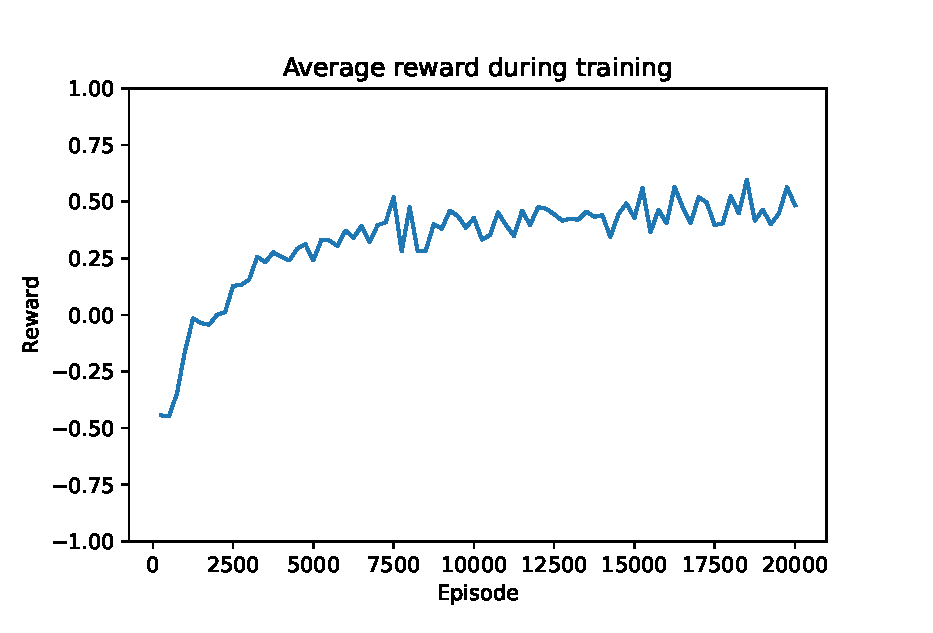
\includegraphics[width = 0.85\linewidth]{code/figures/rewards_Q1.eps}
    \caption{Average reward for every 250 games during training with $\epsilon = 0.1$ against \texttt{Opt(0.5)} for 20'000 games.}
    \label{plot_question1}
\end{figure}

\subsection*{Question 2}
In \Cref{secondplot_question2} we see that for values of $n^{*}$ such that more than half of the training episodes are played with constant $(1-\epsilon_{min})$-greedy policy, after an initial stage where action are chosen randomly more frequently and consequently the reward is lower, the majority of the actions are chosen in a greedy fashion so the average reward increases and approaches the same values seen for $n^{*} = 1$ but with the advantage of having explored more evenly the state space. 
\begin{figure}[H]
    \centering
    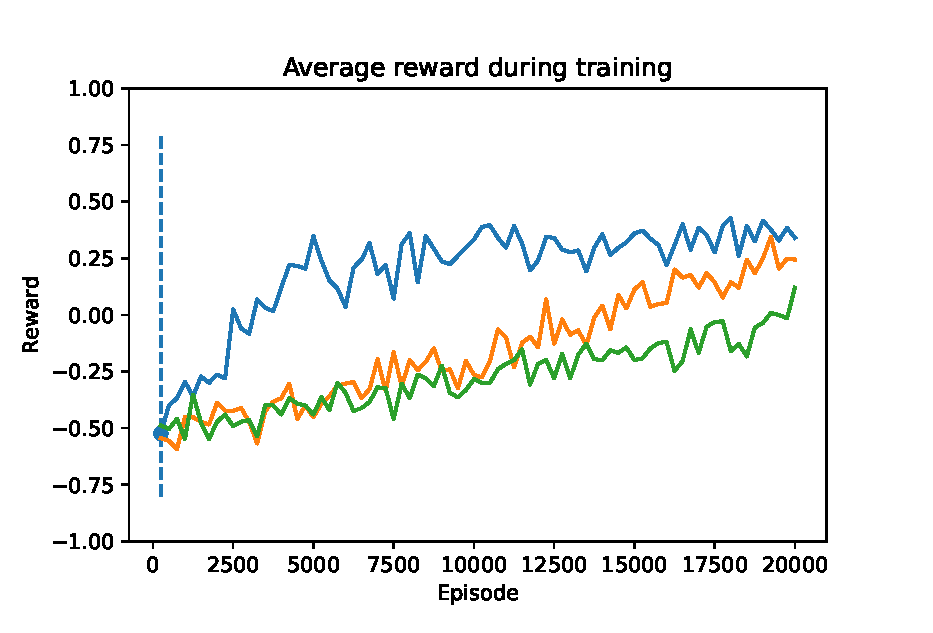
\includegraphics[width = 0.85\linewidth]{code/figures/rewards_n_star_first.eps}
    \caption{Average rewards from training against Opt(0.5) for higher values of $n^{*}$.}
    \label{firstplot_question2}
\end{figure}
In \Cref{firstplot_question2} we see on the other hand that for larger values of $n^{*}$ such that we never reach the constant $(1-\epsilon_{min})$-greedy policy the average reward attains lower values as the agent keeps paying the price of exploration, so it can never reach in terms of performance the $(1-\epsilon_{min})$-greedy agent. For the same reason a stronger decay of $\epsilon$ achieves eventually the same reward as observed in \Cref{plot_question1}.
\begin{figure}[H]
    \centering
    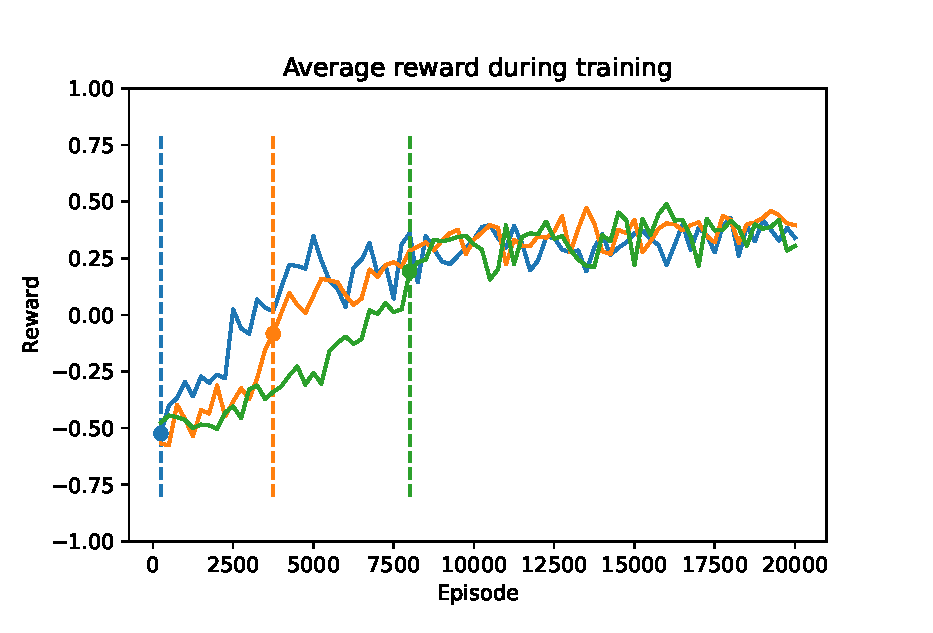
\includegraphics[width = 0.85\linewidth]{code/figures/rewards_n_star_second.eps}
    \caption{Average rewards from training against Opt(0.5) for smaller values of $n^{*}$: the vertical lines correspond approximately to the episode at which the agent starts eventually choosing moves with the minimum rate of exploration (for $n^{*} = 1$ this holds true from the very first episodes).}
    \label{secondplot_question2}
\end{figure}

\subsection*{Question 3}
Due to the high exploration rates, we see in \Cref{firstplot_question3} that for high values of $n^{*}$ major oscillations of \mopt: this instability is caused by the agent not really being able to play as it prioritizes exploring during the learning process. On the other hand, \mrand\  increases slowly, meaning that the agent is not able to take advantage of the opponent's frequent wrong moves and coherently with the low rewards seen before. In \Cref{secondplot_question3} we observe that decreasing majorly $\epsilon$ helps stabilizing the learning process by dumping the oscillations of \mopt\  and increasing faster \mrand\ .
\begin{figure}[H]
    \centering
    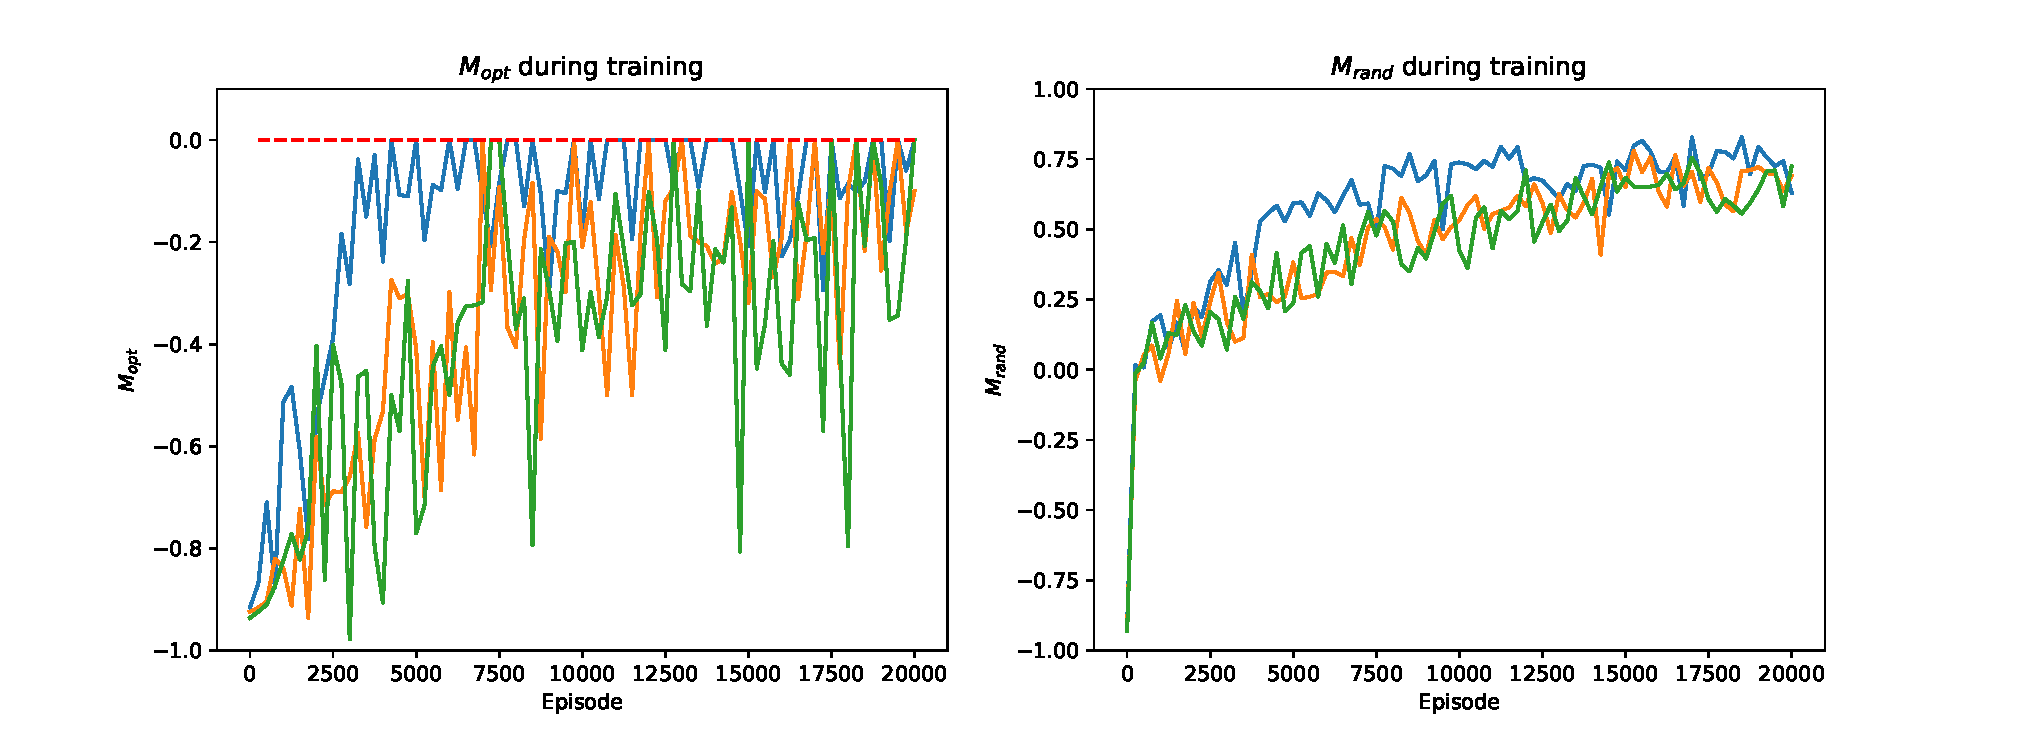
\includegraphics[width=\linewidth]{code/figures/performance_n_star_first.eps}
    \caption{Behaviour of \mopt\  and \mrand\  over the training episodes for high values of $n^{*}$}
    \label{firstplot_question3}
\end{figure}
\begin{figure}[H]
    \centering
    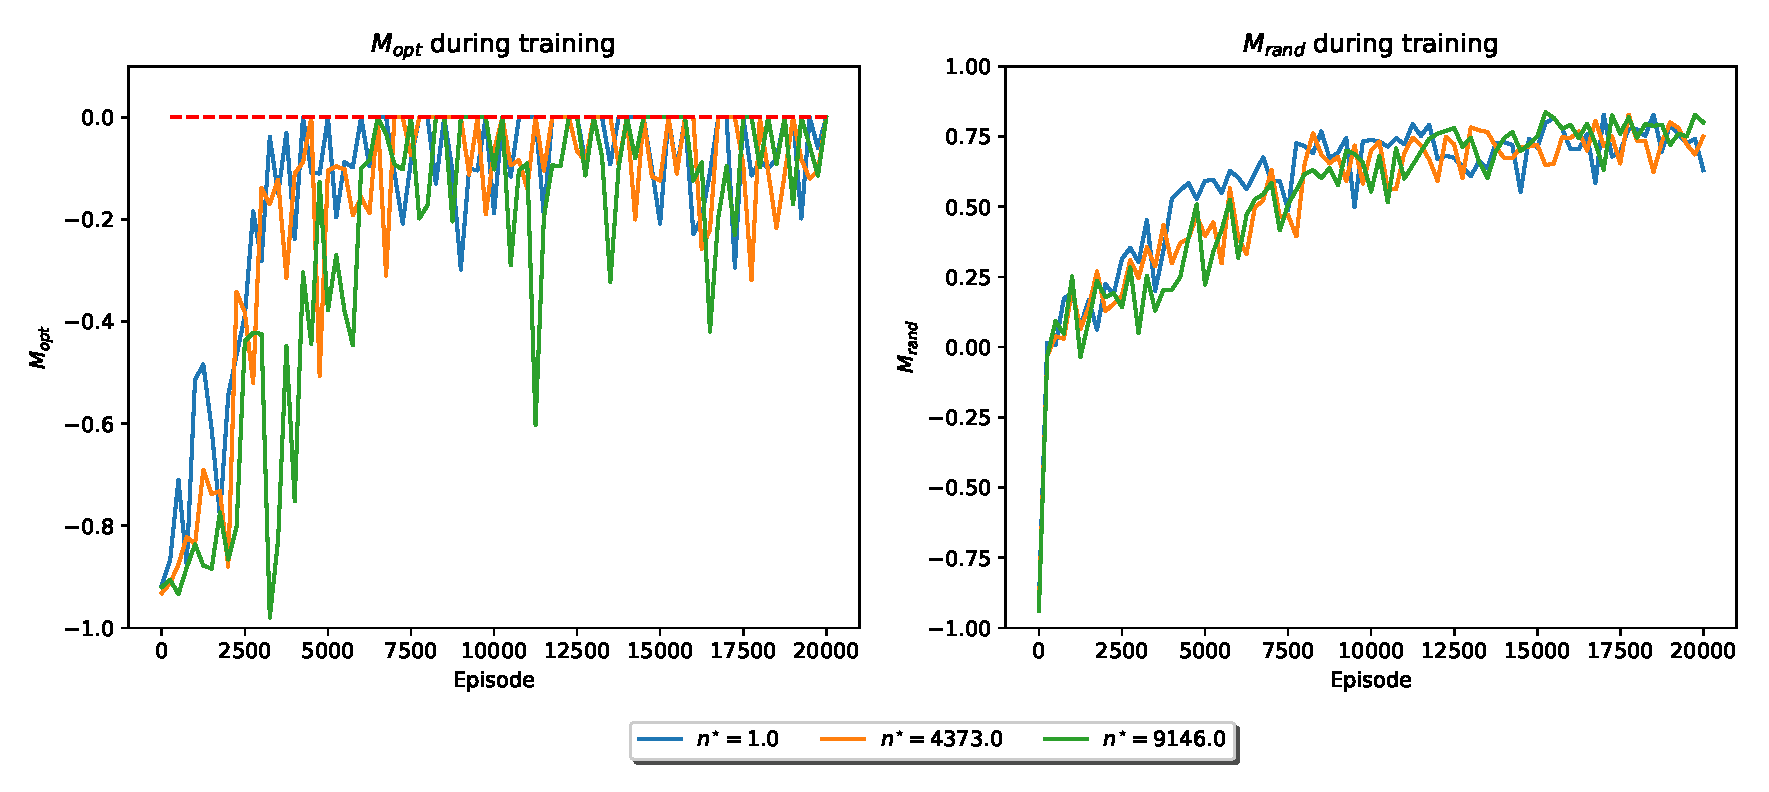
\includegraphics[width=\linewidth]{code/figures/performance_n_star_second.eps}
    \caption{Behaviour of \mopt\  and \mrand\  over the training episodes for small values of $n^{*}$}
    \label{secondplot_question3}
\end{figure}

\subsection*{Question 4}
We compared the performance of the agent trained with Q-learning against \texttt{Opt($\eopt$)} for $\eopt = 0, \, 0.1, \dots, 0.9, \, 1$ and using decreasing exploration with \textcolor{red}{$n^{*} = ...$}. To have a less crowded plot and a clearer comparison, we select the values $\eopt = 0, \, 1, \, 0.5$, which are sufficient to represent the three major behaviours of the training adversary and to show different training trends. \Cref{plot_question4} shows the performance measures \mopt\  and \mrand\  every 250 training episodes.

When training against \texttt{Opt(0)} the agent quickly learns to draw against the optimal player, and \mopt\  reaches 0. However, the performance against the random player \mrand\  does not improve significantly. That is because when playing against the optimal player, there is no possibility of ending up in a win-booking state. Hence, when the agent plays against the random policy and possibly reaches a win-booking state $s_t$, all the $Q$-values $Q(s_t, a)$ are equal to zero (they have never been updated during training), and the agent chooses the next move randomly. 

Conversely, when training against \texttt{Opt(1)} \mrand\  quickly increases, while \mopt\  increases less sharply and without reaching zero. In this case, the agent learns to try to get a $+1$ reward taking advantage of the fact that the opponent can make mistakes, even if this implies sometimes losing the game. Training against \texttt{Opt(0.5)} both \mopt\  and \mrand\  increase significantly. The agent is able to win against the random policy and to draw against the optimal one, but not as good as if trained against \texttt{Opt(0)} or \texttt{Opt(1)} respectively.

In conclusion, the agent learns to gain optimal rewards (in expectation) against the opponent it is trained against. Indeed the optimal $Q$-values depend on the transition probabilities, which vary with the opponent.

\begin{figure}[H]
    \centering
    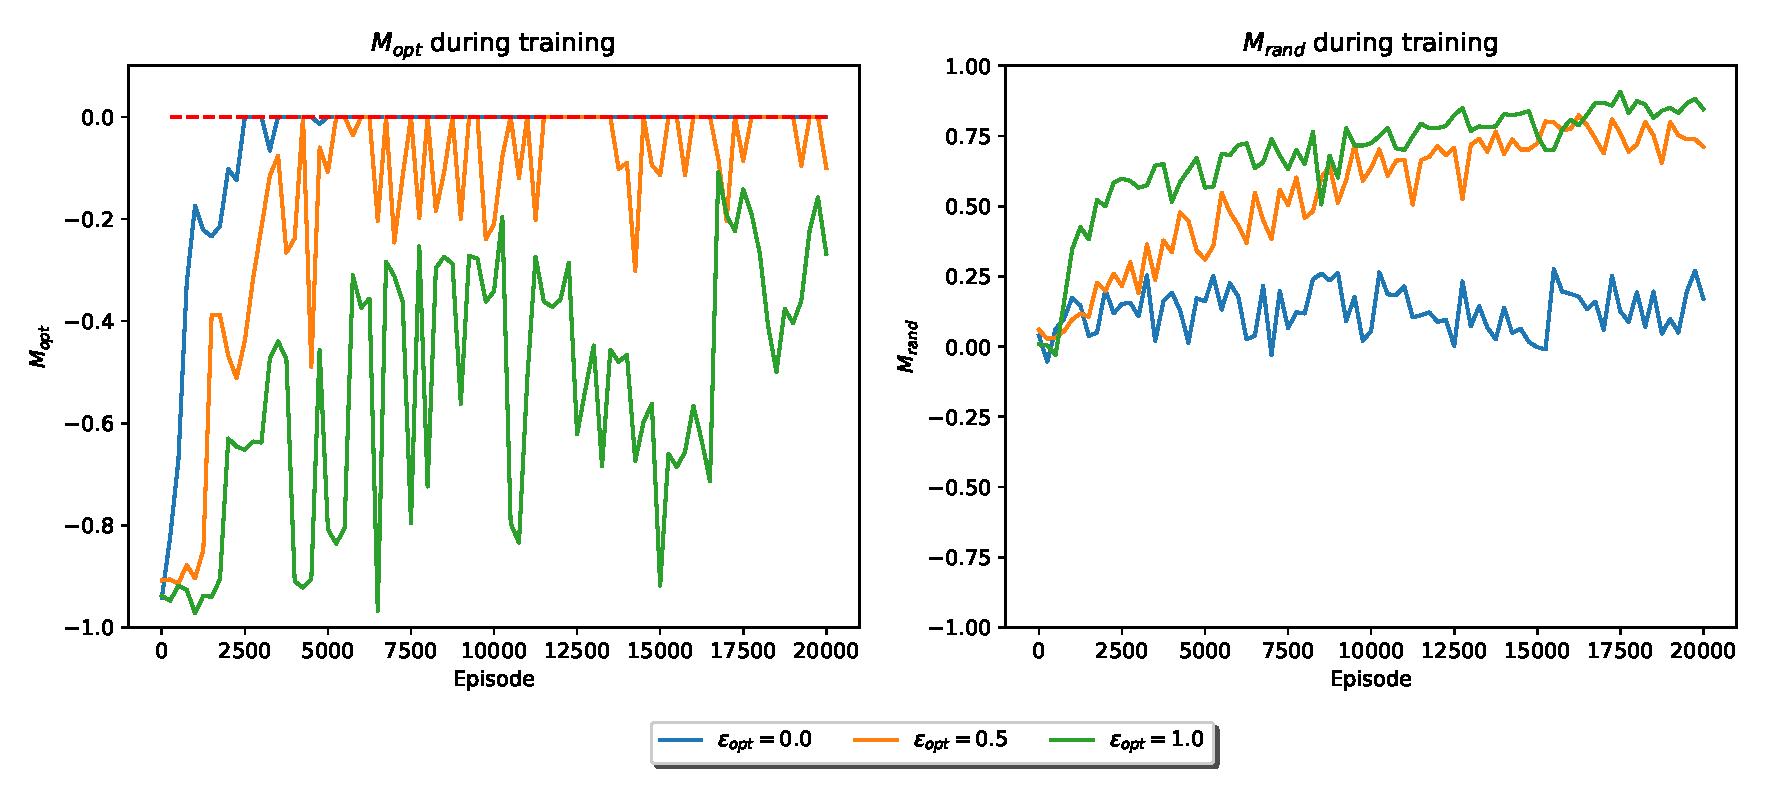
\includegraphics[width=\linewidth]{code/figures/performance_epsilon_opt.eps}
    \caption{Behaviour of \mopt\  and \mrand\  every 250 training episodes for different values of \eopt.}
    \label{plot_question4}
\end{figure}

\subsection*{Question 5}
\subsection*{Question 6}
We claim that $Q_1(s,a)$ and $Q_2(s,a)$ do not have the same values, as suggested by the experimental results shown in \emph{Question 4}.
Indeed, the optimal $Q$-values, i.e. those satisfying the Bellman equation, represent the total expected (discounted) reward and depend on transition probabilities, which are different if playing against \texttt{Opt(1)} or \texttt{Opt(0)}. 

Agent 1 during training never encounters win-booking states, hence at the end of the training $Q_1(s,a)$ is equal to the initialization value for every win-booking state $s$ and every action $a$. This is because the transition probability to any of this states is zero when playing against \texttt{Opt(0)}. Moreover, we expect $Q_1(s,a) = -1$ (possibly discounted by $\gamma$) for actions that make the opponent win (reward $-1$ at the end of the game) and $Q(s,a) = 0$ for all other actions, since Agent 1 can at most draw against \texttt{Opt(0)}. 

On the contrary, Agent 2 encounters win-booking states during training and we expect $Q_2(s,a) = 1$ (possibly discounted by $\gamma$) for actions that make the agent win, hence $Q_2(s,a) \neq Q_1(s,a)$. Furthermore we can expect $Q_2(s,a) \neq Q_1(s,a) -1$ for actions that bring the opponent in a win-booking state, because the \texttt{Opt(1)} plays randomly and might not take the chance to win.

\subsection*{Question 7}


\subsection*{Question 8}

\subsection*{Question 9}
\subsection*{Question 10}
\begin{figure}[H]
\centering
\makebox[\textwidth][c]{
\begin{subfigure}{0.33\textwidth}
\includegraphics[width=\linewidth]{code/figures/heatmaps_0.eps}
\caption{Heatmap 1}
\end{subfigure}\hspace*{\fill}
\begin{subfigure}{0.33\textwidth}
\includegraphics[width=\linewidth]{code/figures/heatmaps_1.eps}
\caption{Heatmap 2}
\end{subfigure}\hspace*{\fill}
\begin{subfigure}{0.33\textwidth}
\includegraphics[width=\linewidth]{code/figures/heatmaps_2.eps}
\caption{Heatmap 3}
\end{subfigure}\hspace*{\fill}}
\caption{Figure caption}
\label{fig_heatmaps}
\end{figure}

\section{Deep Q-Learning}
\subsection*{Question 11}
\subsection*{Question 12}
\subsection*{Question 13}
\subsection*{Question 14}
\subsection*{Question 15}
\subsection*{Question 16}
\subsection*{Question 17}
\subsection*{Question 18}
\subsection*{Question 19}
\subsection*{Question 20}
\subsection*{Question 21}

\section*{Questions to be asked}
\begin{enumerate}
    \item La caption delle figure conta nel conteggio delle parole? Bisogna presentare la risposta alle domande tutta nella caption del plot?
    \item Inizializzazione dei Q-values per la domanda 6
    \item 
\end{enumerate}


\nocite{*}
\printbibliography

\clearpage
\detailtexcount{main}

\end{document}